% =============================================================================
% practica2.tex --- Chapter: Practice 2
% =============================================================================

\documentclass[../../__memoria.tex]{subfiles}

\begin{document}
\standalonecover
\pagestyle{cuerpo}

\graphicspath{{\subfix{../../Imagenes/}}{../../Imagenes/}{\subfix{img/}}{img/}}

\chapter[Práctica 2: Selección de Modelos]{Cuaderno de Laboratorio --- Práctica 2: Selección de Modelos y Regularización}
\chaptermark{Práctica 2}

\section*{Objetivo}
Dominar el protocolo de \textbf{Validación Cruzada (K-Fold)} y comprender cómo la regularización
\textbf{Ridge (L2)} y \textbf{Lasso (L1)} previenen el sobreajuste y ayudan a la \textbf{selección de atributos}.


% =========================================================
% TAREA 1
% =========================================================
\section[Tarea 1: Estabilidad K-Fold]{Tarea 1 --- Estabilidad de la Validación Cruzada (K-Fold)}

\subsection*{Configuración común}
Modelo usado: \textbf{Regresión Lineal (Ridge con $\lambda \approx 0$)} (regresión lineal sin regularización)\\
Métrica: \textbf{RMSE} (RMSE)\\
Semillas: \textbf{\texttt{random\_state} 1, 2, 3, 4 y 5, de forma consecutiva para la tarea 1, y el valor 42 para el resto.}\\

\vspace{0.3cm}
\noindent\textbf{Hipótesis inicial (antes de ejecutar):}
¿Crees que el RMSE será estable al cambiar K? No. Con valores muy bajos de K (ej. K=2), el error dependerá en gran medida de qué datos caigan aleatoriamente en entrenamiento y cuáles en test, provocando alta varianza.

\vspace{0.5cm}

\subsection{Experimento A --- K = 2 (Validación simple): variabilidad entre ejecuciones}

\noindent Ejecuta el modelo \textbf{varias veces} con K=2 (por ejemplo 5--10) y registra el RMSE.
\vspace{0.2cm}
\begin{center}
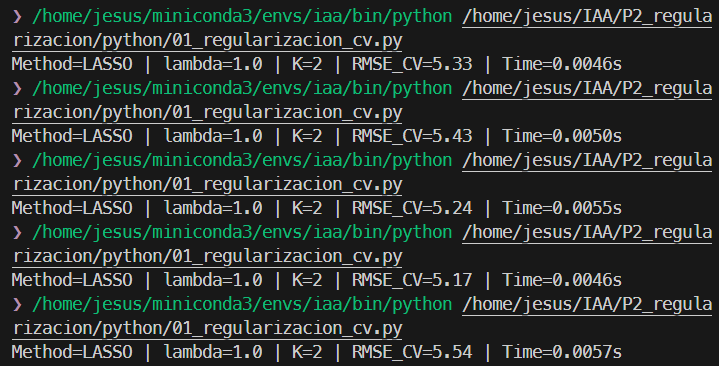
\includegraphics[width=0.90\linewidth]{img/k=2.png}
\end{center}

\noindent\textbf{Registro de resultados (rellena):}
\begin{center}
\begin{tabular}{cc}
\toprule
Ejecución & RMSE \\
\midrule
1 & 5.33 \\
2 & 5.43 \\
3 & 5.24 \\
4 & 5.17 \\
5 & 5.54 \\
\bottomrule
\end{tabular}
\end{center}

\vspace{0.2cm}
\noindent\textbf{Análisis:}
    \begin{itemize}
        \item ¿Por qué el error varía tanto entre ejecuciones? Con K=2 entrenamos solo con el 50\% de los datos, así que según qué muestras caigan en train o test el RMSE cambia bastante. Entre mis 5 ejecuciones el RMSE osciló entre 5.17 y 5.54.
        \item ¿Es fiable esta métrica (con K=2) para tomar una decisión técnica? A mí no me lo parece. Si repito el experimento y obtengo resultados distintos cada vez, no puedo saber si una mejora se debe al modelo o a la partición.
    \end{itemize}

\vspace{0.5cm}

\subsection{Experimento B --- K = 10 (estándar): RMSE más estable}

\noindent Ejecuta el modelo con K=10 y anota el RMSE.
\vspace{0.2cm}
\begin{center}
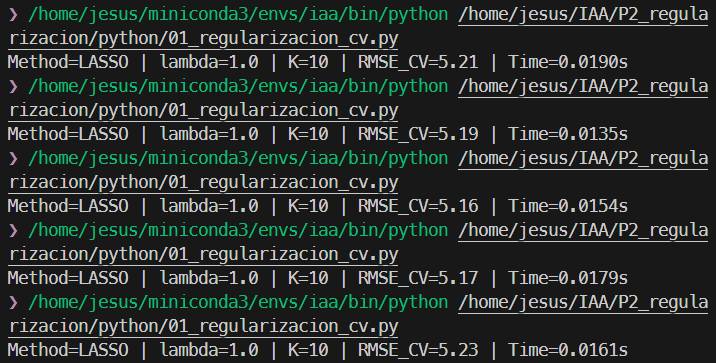
\includegraphics[width=0.90\linewidth]{img/k=10.png}
\end{center}

\noindent RMSE observado (K=10): \textbf{5.19 (Media aprox.)}

\vspace{0.4cm}
\noindent\textbf{Análisis:}
Describe si el resultado parece más estable que en K=2 y por qué. Sí, mucho más estable. Con K=10 el RMSE se movía muy poco (entre 5.16 y 5.23), mientras que con K=2 llegaba a variar hasta 0.37. Tiene sentido: al entrenar con el 90\% de los datos y promediar 10 folds, el resultado depende menos de una partición concreta.

\vspace{0.5cm}

\subsection{Experimento C --- K = 100 (Leave-One-Out): coste vs. precisión}

\noindent Ejecuta el modelo con K=100 (LOOCV) y observa el RMSE y el tiempo.
\vspace{0.2cm}
\begin{center}
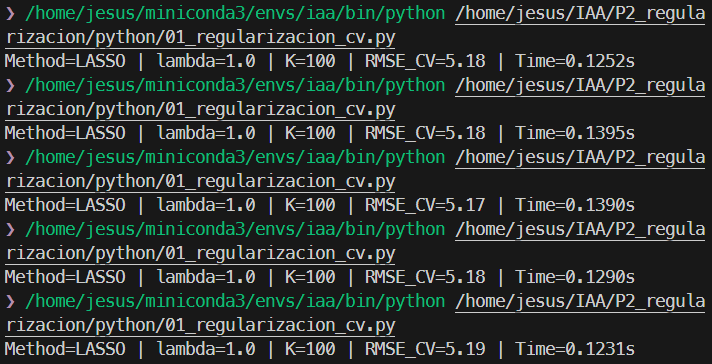
\includegraphics[width=0.90\linewidth]{img/k=100.png}
\end{center}

\noindent RMSE observado (K=100): \textbf{5.18} \quad
Tiempo aproximado: \textbf{0.131s}

\vspace{0.4cm}

\noindent\textbf{Análisis:}
Compara el coste computacional frente a K=10. K=100 tardó 0.131s frente a los 0.016s de K=10, casi 8 veces más. ¿Merece la pena el tiempo extra para mejorar la precisión obtenida? En mi opinión no. El RMSE mejoró solo 0.01 respecto a K=10 (de 5.19 a 5.18), un cambio que no justifica el tiempo adicional.

\vspace{0.5cm}

\subsection{Resumen comparativo (K = 2 vs 10 vs 100)}

\begin{center}
\begin{tabular}{ccc}
\toprule
K & RMSE & Comentario de estabilidad/coste \\
\midrule
2 & 5.17 -- 5.54 & Alta inestabilidad (varianza). Coste muy bajo. \\
10 & 5.16 -- 5.23 & Alta estabilidad. Coste equilibrado y eficiente. \\
100 & 5.17 -- 5.19 & Máxima estabilidad. Coste computacional prohibitivo. \\
\bottomrule
\end{tabular}
\end{center}

\vspace{0.3cm}
\noindent\textbf{Conclusión Tarea 1:}
¿Cuál elegirías para este problema y por qué? Me quedo con K=10. Con K=2 los resultados variaban demasiado entre ejecuciones como para fiarme, y K=100 tardaba mucho para una mejora mínima. K=10 da resultados estables en poco tiempo.

\newpage

% =========================================================
% TAREA 2
% =========================================================
\section[Tarea 2: Ridge vs. Lasso]{Tarea 2 --- Regularización Ridge vs. Lasso (K = 10)}

\subsection*{Configuración}
Fijamos K = 10 y comparamos:
\begin{itemize}
    \item \textbf{Ridge Regression} (penalización L2)
    \item \textbf{Lasso Regression} (penalización L1)
\end{itemize}

\subsection{Ridge (L2) --- \texorpdfstring{$\lambda = 0.1,\, 10,\, 100$}{lambda = 0.1, 10, 100}}

\noindent\textbf{Resultados:} captura el gráfico de barras de coeficientes para cada $\lambda$.
\vspace{0.2cm}
\begin{center}
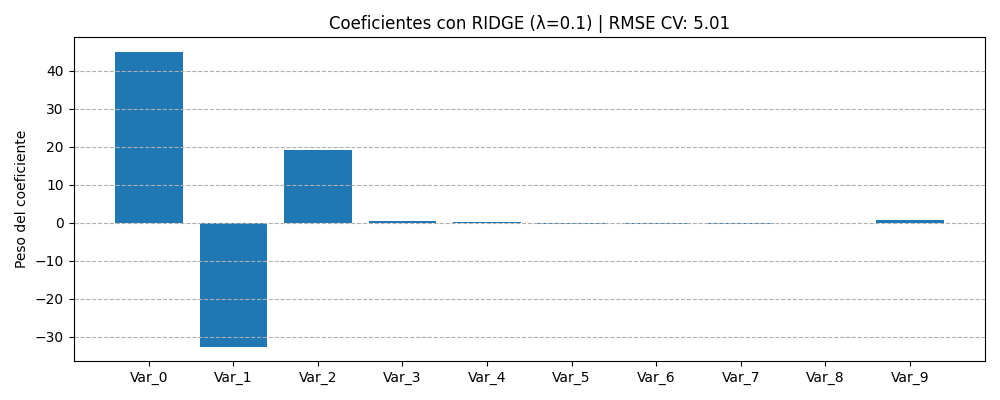
\includegraphics[width=0.90\linewidth]{img/Ra=01.png}
\end{center}
\noindent RMSE Ridge ($\lambda=0.1$): \textbf{5.01}

\vspace{0.4cm}
\begin{center}
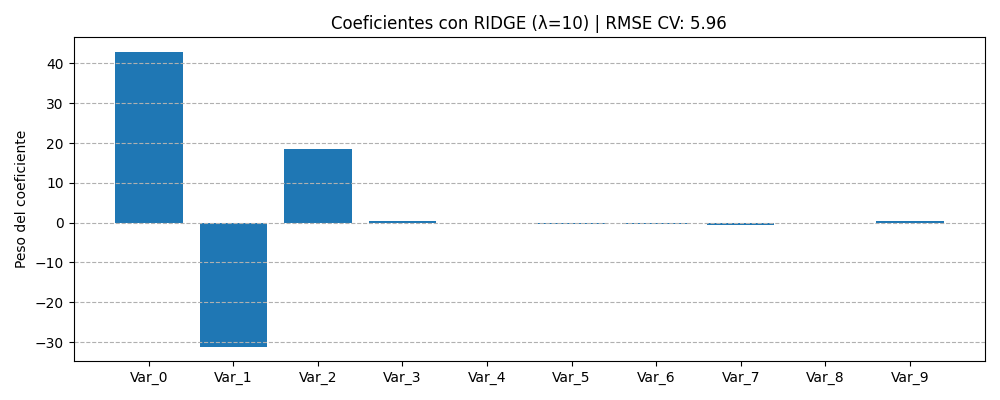
\includegraphics[width=0.90\linewidth]{img/Ra=10.png}
\end{center}
\noindent RMSE Ridge ($\lambda=10$): \textbf{5.96}

\vspace{0.4cm}
\begin{center}
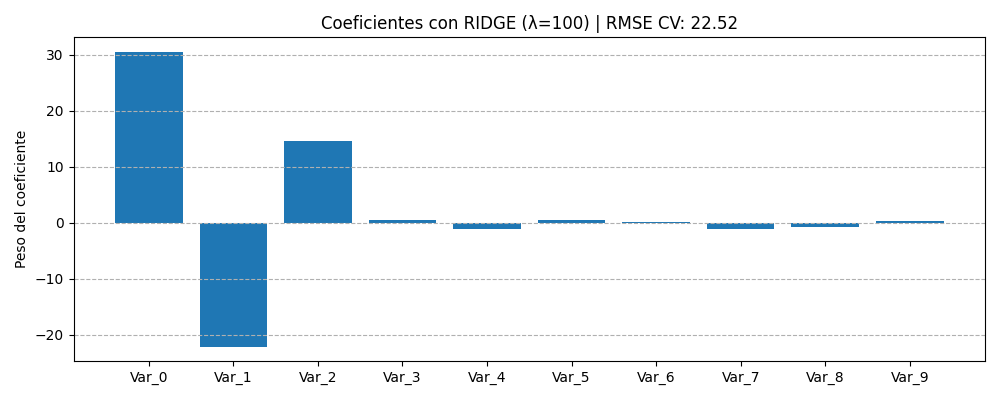
\includegraphics[width=0.90\linewidth]{img/Ra=100.png}
\end{center}
\noindent RMSE Ridge ($\lambda=100$): \textbf{22.52}

\vspace{0.4cm}
\noindent\textbf{Análisis:}
¿Llegan a valer \textbf{cero} los coeficientes de las variables ruidosas?. No llegan a valer cero absoluto. Visualmente en las gráficas parece que algunas como (\texttt{Var\_8} desaparecen, pero técnicamente Ridge (L2) simplemente reduce o "encoge" drásticamente la magnitud de los coeficientes penalizados, distribuyendo el peso entre todos sin llegar a anularlos por completo.

\vspace{0.5cm}

\subsection{Lasso (L1) --- \texorpdfstring{$\lambda = 0.1,\, 10,\, 100$}{lambda = 0.1, 10, 100}}

\noindent\textbf{Resultados:} captura el gráfico de barras de coeficientes para cada $\lambda$.
\vspace{0.2cm}
\begin{center}
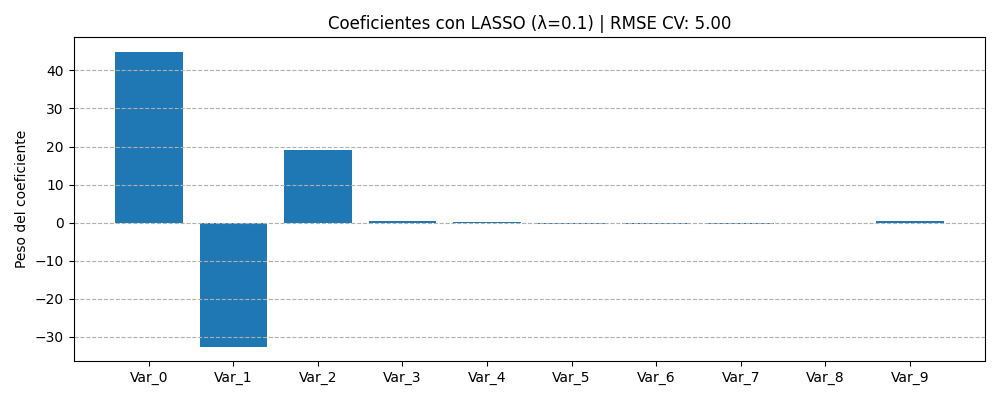
\includegraphics[width=0.90\linewidth]{img/La=01.png}
\end{center}
\noindent RMSE Lasso ($\lambda=0.1$): \textbf{5.00}

\vspace{0.4cm}
\begin{center}
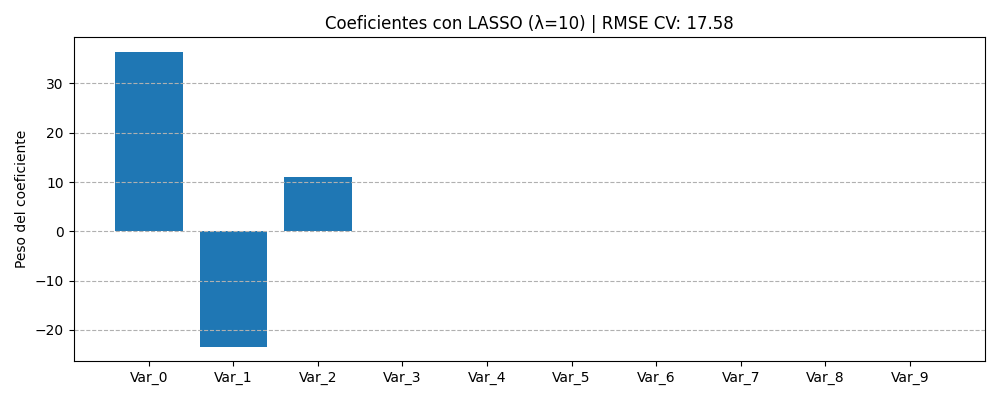
\includegraphics[width=0.90\linewidth]{img/La=10.png}
\end{center}
\noindent RMSE Lasso ($\lambda=10$): \textbf{17.58}

\vspace{0.4cm}
\begin{center}
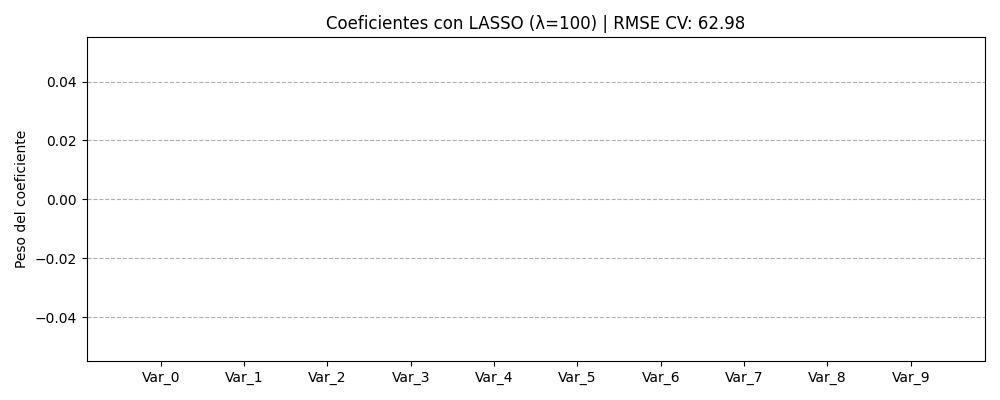
\includegraphics[width=0.90\linewidth]{img/La=100.png}
\end{center}
\noindent RMSE Lasso ($\lambda=100$): \textbf{62.98}

\vspace{0.4cm}
\noindent\textbf{Análisis clave:}
\begin{enumerate}
    \item ¿Para qué $\lambda$ consigue \textbf{Lasso} \textbf{eliminar} las 7 variables ruidosas? Lo probé con varios valores y a partir de $\lambda \approx 1.0$ las variables Var\_3 a Var\_9 se ponían a cero. Por debajo de 0.5 todavía alguna ruidosa se colaba con coeficientes pequeños pero distintos de cero.
    \item Variables con coeficiente distinto de cero (modelo Lasso con ese $\lambda$):\\
    \textbf{Var\_0, Var\_1, Var\_2} — justo las 3 que se usaron para generar los datos.
\end{enumerate}

\vspace{0.5cm}

\subsection{El dilema de la complejidad --- \texorpdfstring{$\lambda$}{lambda} demasiado alto}

\noindent Prueba un valor extremo, por ejemplo $\lambda = 100$, y registra qué ocurre.
\vspace{0.2cm}
\begin{center}
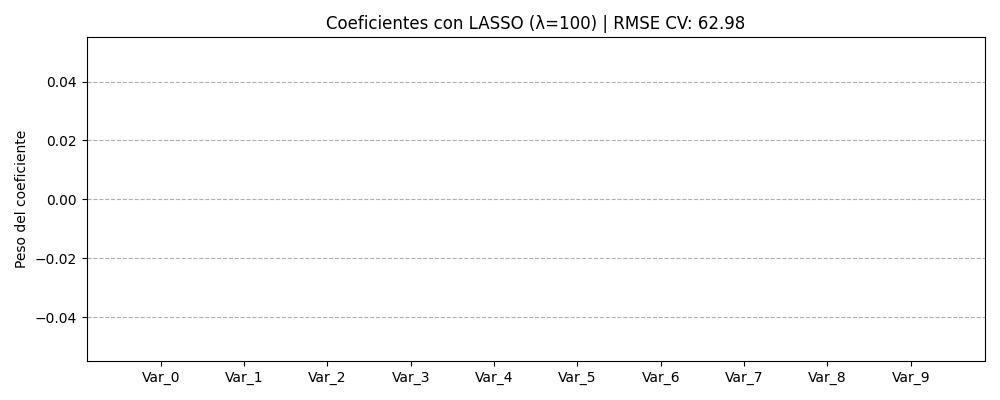
\includegraphics[width=0.90\linewidth]{img/La=100.png}
\end{center}

\noindent RMSE ($\lambda=100$): \textbf{62.98}

\vspace{0.4cm}
\noindent\textbf{Análisis:}
Explica qué ocurre con el RMSE si aplicas un $\lambda$ demasiado alto. El RMSE se dispara exageradamente (hasta 62.98). ¿Estamos ante un caso de \textbf{sesgo alto} o \textbf{varianza alta}? Justifica. Estamos ante un caso evidente de \textbf{sesgo alto (underfitting)}. La penalización es tan severa que el modelo se vuelve excesivamente rígido, empujando todos los coeficientes hacia cero e impidiendo que pueda capturar la señal o patrón real de los datos.

\newpage

% =========================================================
% RETO
% =========================================================
\section{Reto --- El “Cazador de Variables”}

\noindent\textbf{Contexto:} Imagina que cada variable incluida en tu modelo tiene un \textbf{coste de mantenimiento}. Tu objetivo es encontrar el modelo \textbf{más sencillo posible} (menos variables con coeficientes $\neq 0$) que mantenga un RMSE inferior a un umbral:

\[
\text{RMSE} < \textbf{5.50} \quad (\text{umbral asumido})
\]

\vspace{0.3cm}
\noindent\textbf{Mejor solución encontrada (rellena):}
\[
\lambda = \textbf{0.5}
\quad\quad
\text{\#Variables activas} = \textbf{3}
\quad\quad
\text{RMSE} = \textbf{5.03}
\]

\vspace{0.3cm}
\noindent Variables seleccionadas (coeficiente $\neq 0$):
\textbf{Var\_0, Var\_1 y Var\_2}

\vspace{0.5cm}
\begin{center}
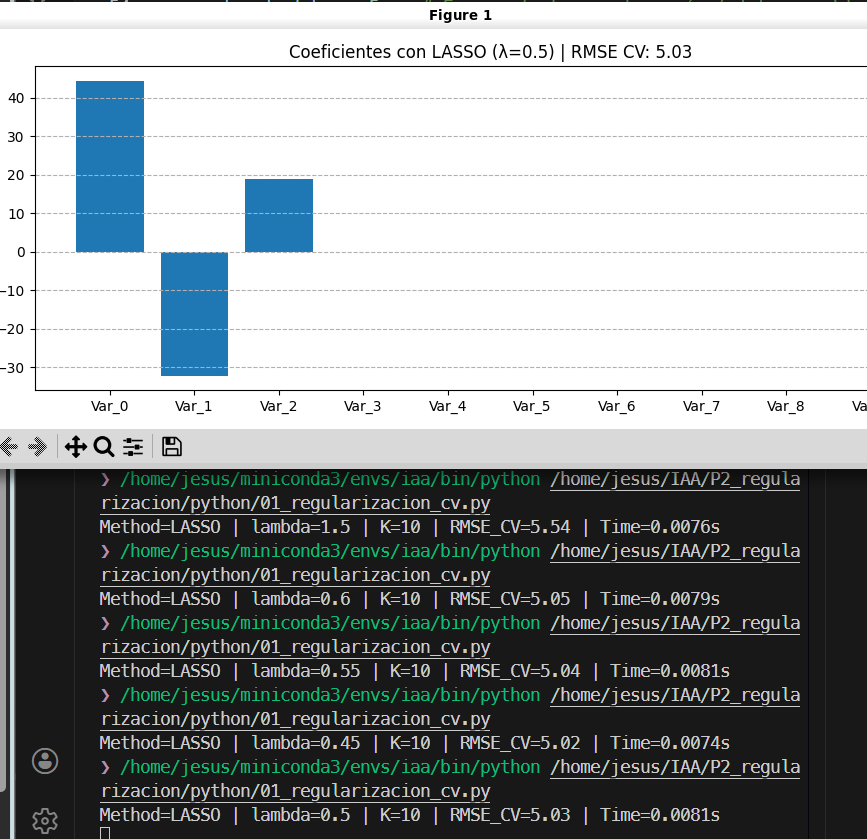
\includegraphics[width=0.90\linewidth]{img/Reto.png}
\end{center}

\vspace{0.3cm}
\noindent\textbf{Justificación técnica (6--10 líneas):}
¿Por qué este modelo es el mejor compromiso entre simplicidad (coste) y rendimiento (RMSE)? 
Tras realizar un ajuste paramétrico fino, $\lambda = 0.5$ demuestra ser el punto de equilibrio óptimo. Logra la máxima simplicidad técnica al descartar completamente los 7 atributos que solo aportaban ruido, minimizando así los futuros costes de mantenimiento e ingesta de datos del modelo. Simultáneamente, conserva un rendimiento excelente con un RMSE de 5.03, el cual es prácticamente idéntico al de modelos menos restrictivos (como $\lambda = 0.1$ con RMSE 5.00). Nos quedamos con la señal real y descartamos el ruido sin penalizar el error.

% =========================================================
% CONCLUSIONES
% =========================================================
\section[Conclusiones]{Conclusiones finales}
Resume en 8--12 líneas lo aprendido sobre:
\begin{itemize}
    \item Estabilidad de K-Fold al variar K (K=2 vs K=10 vs LOOCV).
    \item Diferencias prácticas entre Ridge y Lasso (coeficientes, selección de variables).
    \item Relación entre $\lambda$ grande y el sesgo/varianza.
\end{itemize}

\vspace{0.5cm}
\noindent De la práctica me quedo con dos cosas. Primero, que K=10 es el valor más práctico para validación cruzada: con K=2 los resultados no son fiables y con K=100 se tarda mucho para una mejora mínima. Segundo, la diferencia entre Ridge y Lasso se ve muy clara al probarlos: Ridge reduce los coeficientes de las variables ruidosas pero nunca llega a cero, mientras que Lasso los elimina directamente si subes un poco $\lambda$. Me pareció interesante ver cómo jugando con un solo parámetro ($\lambda$) podía seleccionar automáticamente las 3 variables relevantes y descartar las otras 7. También comprobé que si $\lambda$ es demasiado grande el modelo se vuelve demasiado simple y el error se dispara (underfitting), así que hay que encontrar un punto intermedio.

\end{document}
